% Seccion de optimizacion de la Memoria (OE4), formato de Analisis de algoritmos.
% Requiere: amsmath, amssymb, booktabs, graphicx, algorithm, algpseudocode y las
% cifras de cifras.tex (generadas por ensayos/calibracion/cifras_tex.py).
% Ningun numero de esta seccion se escribe a mano: todos salen de las macros \cal...

\section{Optimización del kit}
\label{sec:calopt}

Esta sección presenta el algoritmo que arma los kits escolares a partir de una
lista ya resuelta contra el catálogo. Primero se analiza el problema y se
enumeran las observaciones que lo hacen difícil
(\cref{sec:calopt-analisis}). A partir de ese análisis se fijan las entradas y
las salidas del algoritmo (\cref{sec:calopt-diseno}), se justifica la
estrategia (\cref{sec:calopt-estrategia}) y se da el seudo-código de las tres
piezas que la componen (\cref{sec:calopt-seudo}). Después se deriva la
complejidad de cada pieza y, de ella y de las mediciones, el umbral que decide
cuándo se enumera (\cref{sec:calopt-complejidad}). La sección cierra con la
calibración de las constantes y las amenazas a la validez
(\cref{sec:calopt-calibracion}).

% ---------------------------------------------------------------------------
\subsection{Análisis del problema}
\label{sec:calopt-analisis}
% ---------------------------------------------------------------------------

Una lista escolar es un conjunto de renglones; cada renglón pide un artículo en
una cantidad. Después de la resolución, cada renglón comprable tiene uno o más
productos del catálogo que lo satisfacen, llamados \emph{candidatos}. El
problema consiste en escoger un candidato por renglón de modo que el kit
resultante sea bueno en varios criterios a la vez. Las observaciones que siguen
fijan la notación y explican de dónde viene la dificultad.

\begin{enumerate}[label=\textbf{O\arabic*.}, ref=O\arabic*]
  \item\label{obs:lineas} Sea $n$ el número de \emph{líneas decidibles}, es
  decir, los renglones comprables que tienen al menos un candidato admisible.
  Un candidato es \emph{admisible} si cumple el atributo que exige el colegio
  (por ejemplo, la marca), o si ningún candidato lo cumple y entonces se admiten
  todos.

  \item\label{obs:conjuntos} Para cada línea $i\in\{1,\dots,n\}$ sea $C_i$ el
  conjunto de sus candidatos admisibles, con cardinal $|C_i|\geq1$. Una
  \emph{asignación} es un vector $\mathbf{x}=(x_1,\dots,x_n)$ con $x_i\in C_i$.

  \item\label{obs:espacio} El \emph{espacio de búsqueda} es el producto
  cartesiano de los conjuntos de candidatos, y su tamaño es el producto de los
  cardinales:
  \[
    \mathcal{S}=C_1\times\cdots\times C_n,\qquad
    S=|\mathcal{S}|=\prod_{i=1}^{n}|C_i| .
  \]
  Si $|C_i|\geq2$ para todas las líneas, $S\geq2^n$, de modo que el espacio
  crece de forma exponencial con el número de líneas. En el corpus de
  \calListas{} listas de \calColegios{} colegios, el espacio más grande tiene
  del orden de $10^{\calEspacioMaxLog}$ asignaciones; \calListasNsga{} listas
  superan el umbral de enumeración de la \cref{sec:calopt-complejidad},
  \calListasExacto{} quedan por debajo y \calListasTriviales{} no tiene ninguna
  decisión que tomar.

  \item\label{obs:objetivos} Cada asignación se evalúa con $M=4$ objetivos:
  el costo $f_1(\mathbf{x})$, que es la suma de precio por unidades a comprar
  y se minimiza; la \emph{fidelidad} $f_2(\mathbf{x})\in[0,1]$, que es el nivel
  de marca promedio normalizado; la \emph{disponibilidad}
  $f_3(\mathbf{x})\in[0,1]$, que es la fracción de líneas con precio conocido;
  y el \emph{personaje} $f_4(\mathbf{x})\in[0,1]$, que es la fracción de líneas
  con el personaje pedido. Los tres últimos se maximizan.

  \item\label{obs:conflicto} Los objetivos están en conflicto: el candidato más
  barato rara vez es el de mejor marca, y el que trae el personaje suele costar
  más. Por eso no existe, en general, una asignación que sea la mejor en los
  cuatro a la vez. Se dice que $\mathbf{x}$ \emph{domina} a $\mathbf{y}$
  ($\mathbf{x}\succ\mathbf{y}$) cuando no es peor en ningún objetivo y es
  estrictamente mejor en al menos uno. El \emph{frente de Pareto}
  $\mathcal{P}\subseteq\mathcal{S}$ es el conjunto de asignaciones que ninguna
  otra domina.

  \item\label{obs:separable} Los cuatro objetivos son sumas (o promedios) de
  términos por línea. Esta estructura permite podar parciales dominados línea
  a línea, y la referencia exacta de los experimentos usa esa poda
  (\cref{sec:calopt-calibracion}). Sin embargo, el número de puntos del frente
  puede crecer con $S$, de modo que la separabilidad no elimina la dificultad
  del problema.

  \item\label{obs:decision} El acudiente necesita un kit, no un frente. Por eso,
  después de calcular $\mathcal{P}$, hay que escoger un punto con sus
  preferencias declaradas: los pesos de los criterios, el tope de gasto y la
  disposición a pagar sobreprecio.
\end{enumerate}

En resumen, lo que hace difícil el problema es la combinación de las
observaciones \ref{obs:espacio} y \ref{obs:conflicto}: el espacio crece de
forma exponencial con las líneas, y como los objetivos están en conflicto la
respuesta es un conjunto de compromisos y no un único óptimo.

% ---------------------------------------------------------------------------
\subsection{Diseño}
\label{sec:calopt-diseno}
% ---------------------------------------------------------------------------

A partir del análisis, el algoritmo recibe las líneas con sus candidatos y las
preferencias del acudiente, y devuelve el frente y el punto recomendado. Las
entradas y las salidas, con sus tipos y dominios, son las siguientes.

\paragraph{Entradas.}
\begin{itemize}
  \item $L=\langle\ell_1,\dots,\ell_n\rangle$: secuencia de líneas decidibles.
  Cada línea $\ell_i$ trae la cantidad pedida $q_i\in\mathbb{N}^{+}$ y el
  conjunto de candidatos $C_i\neq\varnothing$.
  \item Cada candidato $c\in C_i$ es una tupla
  $(p_c,e_c,\nu_c,\pi_c)$ con precio $p_c\in\mathbb{N}\cup\{\bot\}$ en pesos
  colombianos ($\bot$ si no hay precio), unidades por empaque
  $e_c\in\mathbb{N}^{+}$, nivel de marca $\nu_c\in\{0,1,2\}$ (económico,
  confiable, premium) y personaje $\pi_c\in\Sigma^{*}\cup\{\bot\}$.
  \item $\mathbf{w}=(w_{\mathrm{precio}},w_{\mathrm{marca}},w_{\mathrm{calidad}},w_{\mathrm{personaje}})\in\mathbb{R}_{\geq0}^{4}$:
  pesos del acudiente. Si no los declara, se usan los de la encuesta
  (\cref{tab:calopt-constantes}).
  \item $B\in\mathbb{N}^{+}\cup\{\bot\}$: tope de gasto por hijo ($\bot$ si no
  hay tope).
  \item $\sigma\in[0,1]\cup\{\bot\}$: disposición a pagar sobreprecio sobre el
  kit más barato.
  \item $s\in\mathbb{N}$: semilla del generador aleatorio, para que el
  resultado sea reproducible.
\end{itemize}

\paragraph{Salidas.}
\begin{itemize}
  \item $\mathcal{P}\subseteq\mathcal{S}$: conjunto de asignaciones no dominadas,
  cada una con su vector
  $\mathbf{F}(\mathbf{x})=(f_1,f_2,f_3,f_4)\in\mathbb{N}\times[0,1]^3$, ordenado
  por costo ascendente. Es exacto si $S\leq\Lambda$ y aproximado si $S>\Lambda$,
  donde $\Lambda$ es el umbral de enumeración.
  \item $\mathbf{x}^{\star}\in\mathcal{P}\cup\{\bot\}$: asignación recomendada,
  o $\bot$ si ningún punto cumple el tope y el sobreprecio.
\end{itemize}

% ---------------------------------------------------------------------------
\subsection{Estrategia algorítmica}
\label{sec:calopt-estrategia}
% ---------------------------------------------------------------------------

La estrategia tiene dos fases: primero se calcula el frente y después se escoge
un punto sobre él. Para la primera fase hay dos algoritmos, y el tamaño del
espacio decide cuál se usa. Esta subsección explica por qué se aplica cada uno
y en qué orden.

\paragraph{Algoritmo exhaustivo.} La solución de referencia enumera las $S$
asignaciones, calcula sus cuatro objetivos y conserva las no dominadas. Es
correcta por construcción, porque aplica la definición de dominancia sobre todo
el espacio, y no depende de ninguna semilla. Su costo crece con $S$, así que
solo se aplica cuando el espacio es pequeño.

\paragraph{NSGA-II.} Para espacios grandes se usa NSGA-II
\cite{deb_fast_2002}, implementado con pymoo \cite{blank_pymoo_2020}. Es un
algoritmo evolutivo: mantiene una \emph{población} de $N$ asignaciones, y en
cada una de las $G$ \emph{generaciones} produce descendientes por cruce y
mutación y conserva las mejores según el ordenamiento no dominado y la distancia
de apiñamiento. Su costo depende de $N$ y $G$ y no de $S$, a cambio de que el
frente que devuelve sea una aproximación. La población inicial se siembra con
los kits de la heurística por perfil, de modo que el frente aproximado nunca
queda por debajo de ellos. La terminación es por número fijo de generaciones,
porque un criterio de convergencia haría depender el corte del azar de la
corrida.

\paragraph{Conmutación.} Si $S\leq\Lambda$ se enumera y en otro caso se corre
NSGA-II. El umbral $\Lambda$ se elige donde el tiempo de la enumeración alcanza
al del NSGA-II, como se deriva en la \cref{sec:calopt-complejidad}.

\paragraph{Selección a posteriori con MAUT.} La segunda fase escoge un punto del
frente con la teoría de la utilidad multiatributo (MAUT, por sus siglas en
inglés) \cite{keeney_decisions_1976}. Se usa a posteriori, es decir, primero se
calcula el frente y después las preferencias escogen sobre él
\cite[cap.~2.2]{miettinen_nonlinear_1999}. Para cada objetivo se define una
\emph{utilidad normalizada} $u_j:\mathcal{P}\to[0,1]$, lineal sobre el rango
que alcanza el frente:
\[
  u_1(\mathbf{x})=\frac{\max_{\mathcal{P}}f_1-f_1(\mathbf{x})}{\max_{\mathcal{P}}f_1-\min_{\mathcal{P}}f_1},
  \qquad
  u_j(\mathbf{x})=\frac{f_j(\mathbf{x})-\min_{\mathcal{P}}f_j}{\max_{\mathcal{P}}f_j-\min_{\mathcal{P}}f_j}
  \quad(j=2,4),
\]
con $u_j=0$ cuando el rango es nulo. La utilidad del kit es la suma ponderada
\[
  U(\mathbf{x})=\hat w_{\mathrm{precio}}\,u_1(\mathbf{x})
  +(\hat w_{\mathrm{marca}}+\hat w_{\mathrm{calidad}})\,u_2(\mathbf{x})
  +\hat w_{\mathrm{personaje}}\,u_4(\mathbf{x}),
\]
donde $\hat{\mathbf{w}}=\mathbf{w}/\sum_k w_k$ son los pesos renormalizados. La
marca exigida y la calidad pesan las dos sobre la fidelidad porque el frente
mide ambas con el nivel de marca. La forma aditiva supone \emph{independencia
preferencial}, es decir, que la preferencia entre dos valores de un criterio no
depende de los valores fijos de los demás. Solo se consideran los puntos de
máxima disponibilidad, y el tope $B$ y el sobreprecio $\sigma$ son
restricciones duras: $f_1(\mathbf{x})\leq B$ y
$f_1(\mathbf{x})\leq(1+\sigma)\min_{\mathcal{P}}f_1$. Normalizar sobre el
frente, y no sobre un máximo teórico, evita que un rango inalcanzable aplaste
las diferencias reales entre kits.

% ---------------------------------------------------------------------------
\subsection{Seudo-código}
\label{sec:calopt-seudo}
% ---------------------------------------------------------------------------

Esta subsección da tres procedimientos en el orden en que se usan. El
\cref{alg:calopt-exhaustivo} es la línea base exhaustiva. El
\cref{alg:calopt-frente} conmuta entre ella y NSGA-II según el tamaño del
espacio. El \cref{alg:calopt-maut} escoge el punto recomendado sobre el frente.

\begin{algorithm}[htbp]
\caption{Frente exacto por enumeración exhaustiva}
\label{alg:calopt-exhaustivo}
\begin{algorithmic}[1]
\Require líneas $\ell_1,\dots,\ell_n$ con candidatos $C_1,\dots,C_n$
\Ensure frente de Pareto exacto $\mathcal{P}$
\Procedure{FrenteExhaustivo}{$C_1,\dots,C_n$}
  \State $V\gets\varnothing$ \Comment{vectores objetivo distintos}
  \ForAll{$\mathbf{x}\in C_1\times\cdots\times C_n$} \Comment{$S$ iteraciones}
    \State $\mathbf{v}\gets\mathbf{F}(\mathbf{x})$ \Comment{$\Theta(n)$ por asignación}
    \If{$\mathbf{v}\notin V$} $V\gets V\cup\{(\mathbf{v},\mathbf{x})\}$ \EndIf
  \EndFor
  \State $\mathcal{P}\gets\varnothing$
  \ForAll{$(\mathbf{v},\mathbf{x})\in V$} \Comment{filtro de no dominados}
    \If{$\nexists(\mathbf{w},\cdot)\in V:\ \mathbf{w}\succ\mathbf{v}$} \Comment{$O(|V|\,M)$}
      \State $\mathcal{P}\gets\mathcal{P}\cup\{(\mathbf{v},\mathbf{x})\}$
    \EndIf
  \EndFor
  \State \Return $\mathcal{P}$ ordenado por $(f_1,-f_2,-f_3,-f_4)$
\EndProcedure
\end{algorithmic}
\end{algorithm}

\begin{algorithm}[htbp]
\caption{Conmutación entre el frente exacto y NSGA-II}
\label{alg:calopt-frente}
\begin{algorithmic}[1]
\Require candidatos $C_1,\dots,C_n$; umbral $\Lambda$; semilla $s$
\Ensure frente $\mathcal{P}$ (exacto si $S\leq\Lambda$)
\Procedure{Frente}{$C_1,\dots,C_n,\Lambda,s$}
  \State $S\gets\prod_{i=1}^{n}|C_i|$
  \If{$S\leq1$} \Return $\varnothing$ \Comment{no hay decisión que tomar}
  \ElsIf{$S\leq\Lambda$}
    \State \Return \Call{FrenteExhaustivo}{$C_1,\dots,C_n$}
  \EndIf
  \State $N\gets\mathrm{par}\bigl(\min(a\,N_{\max},\max(a\,N_{\min},12\,a\,n))\bigr)$ \Comment{población}
  \State $G\gets\min(b\,G_{\max},\max(b\,G_{\min},20\,b\log_{10}S))$ \Comment{generaciones}
  \State $Q_0\gets$ kits heurísticos y escalera de costo marginal
  \State $Q_0\gets Q_0\cup\{$asignaciones al azar con semilla $s\}$ hasta $|Q_0|=N$
  \For{$g\gets1$ \textbf{hasta} $G$}
    \State $R\gets Q_{g-1}\cup\textsc{CruceYMutación}(Q_{g-1})$ \Comment{$2N$ individuos}
    \State $\mathcal{F}_1,\mathcal{F}_2,\dots\gets\textsc{OrdenNoDominado}(R)$ \Comment{$O(MN^2)$}
    \State $Q_g\gets$ los $N$ mejores de $R$ por frente y apiñamiento
  \EndFor
  \State \Return no dominados de $Q_G\cup Q_0$ \Comment{la siembra entra al filtro final}
\EndProcedure
\end{algorithmic}
\end{algorithm}

\begin{algorithm}[htbp]
\caption{Selección a posteriori por utilidad aditiva (MAUT)}
\label{alg:calopt-maut}
\begin{algorithmic}[1]
\Require frente $\mathcal{P}$; pesos $\mathbf{w}$; tope $B$; sobreprecio $\sigma$
\Ensure asignación recomendada $\mathbf{x}^{\star}$ o $\bot$
\Procedure{ElegirMAUT}{$\mathcal{P},\mathbf{w},B,\sigma$}
  \If{$\mathcal{P}=\varnothing$} \Return $\bot$ \EndIf
  \State $\mathcal{P}\gets\{\mathbf{x}\in\mathcal{P}: f_3(\mathbf{x})=\max_{\mathcal{P}}f_3\}$ \Comment{solo lo surtible}
  \State $\hat{\mathbf{w}}\gets\mathbf{w}/\sum_k w_k$ \Comment{pesos que suman 1}
  \State calcular $\min_{\mathcal{P}}f_j$ y $\max_{\mathcal{P}}f_j$ para $j=1,2,4$
  \State $K\gets\mathcal{P}$
  \If{$\sigma\neq\bot$} $K\gets\{\mathbf{x}\in K: f_1(\mathbf{x})\leq(1+\sigma)\min_{\mathcal{P}}f_1\}$ \EndIf
  \If{$B\neq\bot$} $K\gets\{\mathbf{x}\in K: f_1(\mathbf{x})\leq B\}$ \EndIf
  \If{$K=\varnothing$} \Return $\bot$ \Comment{ningún kit cumple las restricciones}
  \EndIf
  \State \Return $\arg\max_{\mathbf{x}\in K}\bigl(U(\mathbf{x}),-f_1(\mathbf{x}),f_2(\mathbf{x}),f_4(\mathbf{x})\bigr)$ \Comment{orden lexicográfico}
\EndProcedure
\end{algorithmic}
\end{algorithm}

% ---------------------------------------------------------------------------
\subsection{Complejidad}
\label{sec:calopt-complejidad}
% ---------------------------------------------------------------------------

Esta subsección deriva primero el costo de cada procedimiento, después
compara el exhaustivo con NSGA-II y, a partir de ambas cosas y de las
mediciones, fija el umbral $\Lambda$.

\paragraph{Exhaustivo.} El primer ciclo del \cref{alg:calopt-exhaustivo} visita
las $S$ asignaciones y evalúa en cada una $M$ objetivos que suman $n$
términos, de modo que cuesta $\Theta(S\cdot n)$; si se cuenta por objetivo,
$\Theta(S\cdot M)$ evaluaciones de objetivo con $n$ fijo. El filtro compara
cada uno de los $U\leq S$ vectores distintos con todos los demás, con un costo
de $O(U^2M)$ en el peor caso. Kung, Luccio y Preparata
\cite{kung_finding_1975} reducen el filtro a $O(U\log^{M-2}U)$, pero con $M=4$
y los $U$ observados la versión por pares ya resulta más rápida que la
evaluación misma. El total es
\[
  T_{\mathrm{exh}}(S)=\Theta\Bigl(\prod_{i=1}^{n}|C_i|\cdot M\Bigr)+O(U^2M),
  \qquad U\leq S .
\]

\paragraph{NSGA-II.} Cada generación del \cref{alg:calopt-frente} ordena por no
dominancia $2N$ individuos, con un costo $O(MN^2)$ \cite{deb_fast_2002}, y
evalúa $N$ descendientes con un costo $O(Nn)$. Con $G$ generaciones el total es
\[
  T_{\mathrm{NSGA}}=O\bigl(G\cdot M\cdot N^2\bigr),
\]
que no depende de $S$. Como $N\leq a N_{\max}$ y $G\leq b G_{\max}$, el costo
está acotado por una constante para cualquier lista. A cambio, el resultado es
una aproximación.

\paragraph{MAUT.} El \cref{alg:calopt-maut} recorre el frente un número
constante de veces, así que cuesta $O(|\mathcal{P}|\,M)$. Es despreciable frente
a la construcción del frente.

\paragraph{Umbral teórico.} El umbral es el valor de $S$ donde los dos costos
se igualan. Si se comparan las operaciones dominantes,
$S\cdot M=G\cdot M\cdot N^2$, el cruce queda en $S^{\ast}=G N^2$; si se compara
el filtro por pares del exhaustivo en su peor caso, $S^2M=GMN^2$, queda en
$S^{\ast}=N\sqrt{G}$. Con la configuración elegida
(\cref{sec:calopt-calibracion}) y $n=\calNTipico$ líneas, que es la mediana
de los subproblemas cercanos al umbral, la población es $N=\calPobTipica$ y
las generaciones son $G=\calGenTipica$. Entonces la primera cota da
$GN^2=\calSCuadrado$ ($2^{\calSCuadradoLog}$) y la segunda da
$N\sqrt{G}\approx\calSTeorico$ ($2^{\calSTeoricoLog}$); como referencia, el
NSGA-II hace $NG=\calSEvals$ evaluaciones ($2^{\calSEvalsLog}$). El umbral
queda, por tanto, entre $2^{\calSTeoricoLog}$ y $2^{\calSCuadradoLog}$. La
teoría no lo precisa más porque las constantes de cada operación son
distintas: evaluar una asignación en Python cuesta mucho más que comparar dos
vectores dentro de pymoo, y el filtro rara vez llega a su peor caso porque
$U<S$. Por eso el umbral se fija con la medición.

\paragraph{Umbral medido.} Para medirlo se armaron \calSubproblemas{}
subproblemas con líneas reales, con espacios $S\in[2^{b},2^{b+1})$ para
$b=\calNivelMin,\dots,\calNivelMax$, y en cada uno se midió el tiempo de pared
de la enumeración y del NSGA-II en serie. La enumeración se midió hasta
$b=\calNivelMaxExacto$; más arriba ya pasaba de dos minutos y no se corrió. Un
ajuste por mínimos cuadrados en escala log-log sobre los
\calSubproblemasExacto{} subproblemas enumerados da
\[
  t_{\mathrm{exh}}(S)\approx\calConstante\cdot S^{\calExponente}\ \mathrm{s},
\]
con desviación estándar del residuo logarítmico de \calSdResiduo. El exponente
es mayor que 1 porque el filtro de no dominados crece más rápido que la
evaluación. La mediana del tiempo del NSGA-II con la configuración elegida es
de \calTNsgaElegidaMediana~s, y el ajuste la alcanza en
$S\approx\calCruceElegida$ ($2^{\calCruceElegidaLog}$). Si se toma el percentil
95 del ajuste, es decir, una enumeración lenta, el cruce baja a
$S\approx\calCruceElegidaP$ ($2^{\calCruceElegidaPLog}$). La
\cref{tab:calopt-umbral} resume los tiempos por nivel con la configuración de
partida y la \cref{fig:calopt-umbral} los muestra junto con el ajuste.

\begin{table}[htbp]
\centering
\caption{Tiempo de pared de la enumeración exhaustiva y del NSGA-II con la
configuración de partida y con la elegida, por nivel $b$ del espacio
($S\in[2^b,2^{b+1})$). «Exacto más rápido» y «HV mínimo» se refieren a la
configuración elegida.
Fuente: \texttt{umbral.json} y \texttt{umbral\_elegida.json}; \calSubproblemas{} subproblemas,
\calSemillasHV{} semillas por subproblema para el hipervolumen; máquina
\calCPU{} con \calRAM~GiB.}
\label{tab:calopt-umbral}
\small
\begin{tabular}{rrrrrrrr}
\toprule
 & & \multicolumn{2}{c}{exacto (s)} & \multicolumn{2}{c}{NSGA-II, mediana (s)} & & \\
$b$ & subproblemas & mediana & máx. & partida & elegida & exacto más rápido & HV mínimo \\
\midrule
6 & 5 & 0{,}001 & 0{,}001 & 1{,}382 & 0{,}258 & 5 & 1{,}0000 \\
7 & 5 & 0{,}002 & 0{,}003 & 0{,}703 & 0{,}197 & 5 & 1{,}0000 \\
8 & 5 & 0{,}005 & 0{,}011 & 0{,}388 & 0{,}163 & 5 & 1{,}0000 \\
9 & 5 & 0{,}015 & 0{,}020 & 0{,}372 & 0{,}188 & 5 & 1{,}0000 \\
10 & 5 & 0{,}032 & 0{,}058 & 0{,}439 & 0{,}211 & 5 & 1{,}0000 \\
11 & 5 & 0{,}089 & 0{,}294 & 0{,}401 & 0{,}183 & 3 & 0{,}9998 \\
12 & 5 & 0{,}354 & 0{,}731 & 0{,}420 & 0{,}223 & 1 & 0{,}9999 \\
13 & 5 & 1{,}301 & 2{,}457 & 0{,}461 & 0{,}239 & 0 & 1{,}0000 \\
14 & 5 & 1{,}420 & 7{,}553 & 0{,}581 & 0{,}288 & 0 & 0{,}9996 \\
15 & 3 & 11{,}912 & 25{,}134 & 0{,}632 & 0{,}337 & 0 & 0{,}9998 \\
16 & 3 & 48{,}534 & 142{,}993 & 0{,}538 & 0{,}274 & 0 & 0{,}9997 \\
17 & 3 & 27{,}650 & 179{,}797 & 0{,}642 & 0{,}356 & 0 & 1{,}0000 \\
18 & 3 & --- & --- & 0{,}712 & 0{,}356 & 0 & 0{,}9999 \\
\bottomrule

\end{tabular}
\end{table}

\begin{figure}[htbp]
\centering
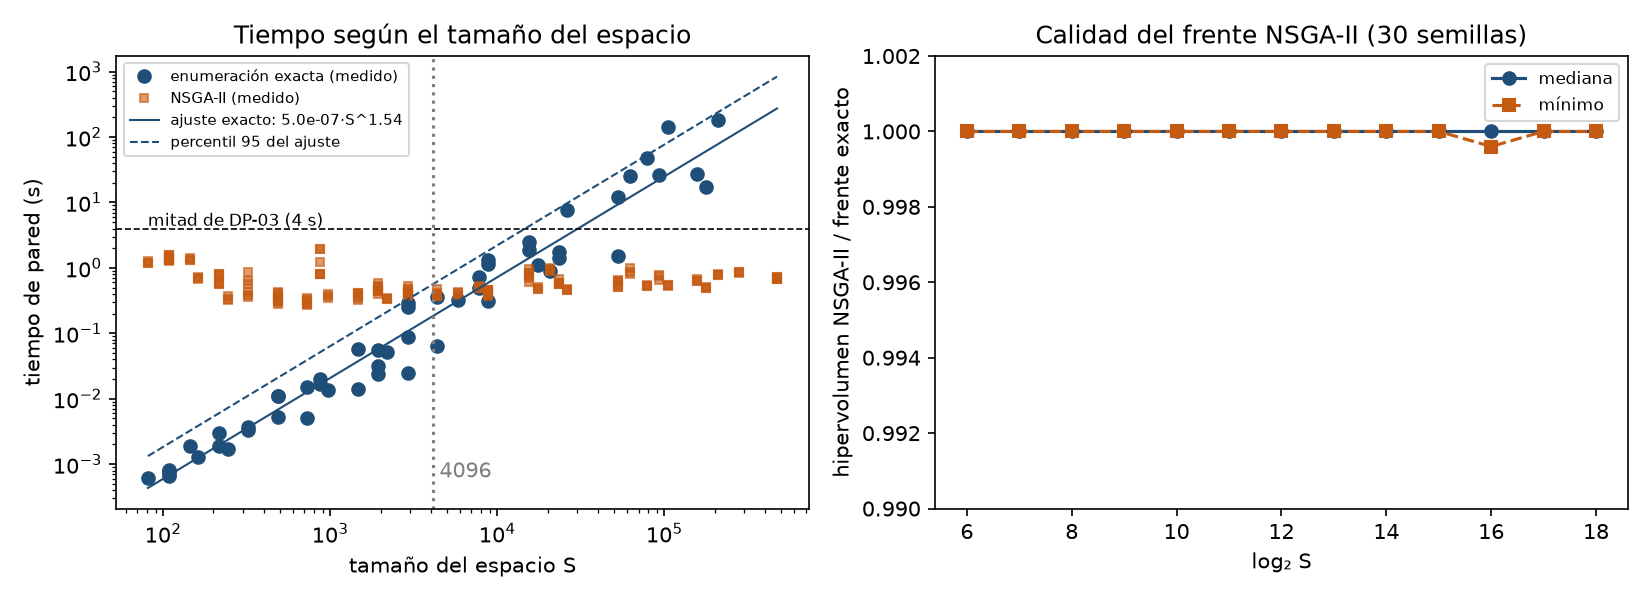
\includegraphics[width=\linewidth]{umbral.png}
\caption{Izquierda: tiempo de la enumeración exacta y del NSGA-II según $S$,
con el ajuste $t\approx\calConstante\cdot S^{\calExponente}$ y su percentil
95. Derecha: razón de hipervolumen del NSGA-II contra el frente exacto, mediana
y mínimo por nivel. Fuente: \texttt{umbral.json}, $n=\calSubproblemas$
subproblemas; los valores están en la \cref{tab:calopt-umbral}.}
\label{fig:calopt-umbral}
\end{figure}

A partir de esas dos cifras se fija $\Lambda=\calLimite=2^{\calLimiteLog}$,
que queda entre el cruce del percentil 95 y el de la mediana y dentro del rango
que predice la teoría. Por debajo del umbral la enumeración fue más rápida que
el NSGA-II calibrado en \calExactoGanaBajoElegida{} subproblemas y tardó como
mucho \calExactoMaxBajo~s; por encima lo fue solo en
\calExactoGanaSobreElegida. Un umbral menor perdería el frente exacto en
espacios donde enumerar todavía es barato, y uno mayor haría esperar segundos
por un frente que el NSGA-II encuentra casi igual en una fracción de ese
tiempo.

\paragraph{Comparación con el exhaustivo.} El exhaustivo da el frente óptimo,
pero su tiempo crece como $S^{\calExponente}$ y pasa de dos minutos cerca de
$2^{\calNivelMaxExacto}$, mientras que una lista real llega a
$10^{\calEspacioMaxLog}$. El NSGA-II tarda menos de un segundo en todos los
niveles medidos. La pérdida de calidad es pequeña: sobre
\calCorridasHV{} corridas (subproblemas por semillas), la razón de hipervolumen
contra el frente exacto tuvo mediana \calRazonHVMediana{} y mínimo
\calRazonHVMin. El \emph{hipervolumen} es el volumen del espacio de objetivos
que domina un frente hasta un punto de referencia \cite{zitzler_multiobjective_1999};
aquí los cuatro ejes se normalizan a $[0,1]$ y la referencia es $1{,}1$ en cada
eje. Una razón de 1 significa que el NSGA-II encontró un frente tan bueno como
el exacto.

% ---------------------------------------------------------------------------
\subsection{Calibración y amenazas a la validez}
\label{sec:calopt-calibracion}
% ---------------------------------------------------------------------------

Esta subsección explica de dónde sale cada constante del optimizador, en este
orden: los pesos por omisión, la población y las generaciones del NSGA-II, el
umbral de similitud de la resolución y la sensibilidad del kit recomendado. Al
final se resumen las constantes en la \cref{tab:calopt-constantes} y se
declaran las amenazas a la validez. Todos los experimentos corrieron en un
\calCPU{} con \calNucleos{} núcleos y \calRAM~GiB de memoria, con Python
\calPython{} y pymoo \calPymoo.

\paragraph{Pesos por omisión.} La pregunta P21 de la encuesta pide a cada
acudiente ordenar los cuatro criterios de mayor a menor importancia. Se le dan
4 puntos al primero y 1 al último, y el peso de cada criterio es su puntaje
medio dividido entre 10, de modo que los cuatro suman 1. Con
\calEncuestados{} respuestas y un intervalo bootstrap percentil del 95\,\%
\cite{efron_bootstrap_1979} con \calRemuestreos{} remuestreos, los pesos son:
precio \calWPrecio{} [\calWPrecioBajo; \calWPrecioAlto], marca exigida
\calWMarca{} [\calWMarcaBajo; \calWMarcaAlto], calidad \calWCalidad{}
[\calWCalidadBajo; \calWCalidadAlto] y personaje \calWPersonaje{}
[\calWPersonajeBajo; \calWPersonajeAlto]. Reemplazan a los valores anteriores
del código (\calWPrecioAntes; \calWMarcaAntes; \calWCalidadAntes;
\calWPersonajeAntes), que no venían de ninguna medición. Los tres primeros
intervalos se solapan, de modo que la encuesta no permite ordenar precio, marca
y calidad entre sí; solo el personaje queda claramente por debajo.

\paragraph{Población y generaciones.} Las fórmulas de partida eran
$N=\mathrm{par}(\min(\calPobMax,\max(\calPobMin,12n)))$ y
$G=\min(\calGenMax,\max(\calGenMin,20\log_{10}S))$. La calibración multiplica
la población por $a$ y las generaciones por $b$, con $a,b\in\{\calFactores\}$,
y mide la razón de hipervolumen contra el frente exacto. La partición es por
colegio, porque dos grados de un mismo colegio comparten productos y marcas, y
mezclarlos entre ajuste y prueba inflaría el resultado. De las
\calGrandes{} listas que corren NSGA-II, \calPrueba{} listas de
\calColegiosPrueba{} colegios se apartaron como prueba antes de mirar nada. El
resto se repartió en \calPliegues{} pliegues por colegio (\calPlieguesListas{}
listas), con \calSemillasCV{} semillas por lista. La regla escoge la
configuración más barata en evaluaciones ($N\cdot G$) cuyo hipervolumen medio
no baja más de \calUmbralHV{} del mejor de la rejilla. Aplicada sobre todos
los pliegues, la regla eligió $a=\calA$ y $b=\calB$, de modo que en
producción la población es
$N=\mathrm{par}(\min(\calPobProdMax,\max(\calPobProdMin,\calPobProdLinea\,n)))$
y las generaciones son
$G=\min(\calGenProdMax,\max(\calGenProdMin,\calGenProdDecada\log_{10}S))$.
Al aplicar la regla dejando fuera cada pliegue, eligió la misma configuración
en \calPlieguesIguales{} pliegues, y la elegida quedó dentro del margen en el
pliegue apartado en \calPlieguesDentro. El pliegue que difiere escogió una
configuración todavía más barata, y esa configuración quedó por fuera del margen
en su pliegue apartado, lo que indica que reducir más el presupuesto ya cuesta
calidad. La \cref{tab:calopt-rejilla} da la rejilla completa y la
\cref{fig:calopt-rejilla} la muestra.

\begin{table}[htbp]
\centering
\caption{Rejilla de población ($a$) y generaciones ($b$) sobre los pliegues de
validación. $\star$: configuración elegida; $\circ$: configuración de partida.
Fuente: \texttt{calibracion\_nsga.json}; $n=\calCVListas$ listas,
\calSemillasCV{} semillas por lista.}
\label{tab:calopt-rejilla}
\small
\begin{tabular}{rrrrrrc}
\toprule
$a$ & $b$ & evaluaciones medias & HV medio & HV mínimo por lista & tiempo medio (s) & \\
\midrule
0{,}25 & 0{,}25 & 1\,231 & 0{,}9960 & 0{,}9711 & 0{,}29 &  \\
0{,}25 & 0{,}50 & 2\,475 & 0{,}9973 & 0{,}9708 & 0{,}57 &  \\
0{,}25 & 1{,}00 & 4\,963 & 0{,}9971 & 0{,}9615 & 1{,}18 &  \\
0{,}25 & 2{,}00 & 9\,937 & 0{,}9975 & 0{,}9725 & 2{,}30 &  \\
0{,}50 & 0{,}25 & 2\,453 & 0{,}9986 & 0{,}9904 & 0{,}48 &  \\
0{,}50 & 0{,}50 & 4\,931 & 0{,}9998 & 0{,}9970 & 1{,}01 & $\star$ \\
0{,}50 & 1{,}00 & 9\,890 & 1{,}0000 & 0{,}9981 & 2{,}01 &  \\
0{,}50 & 2{,}00 & 19\,800 & 1{,}0000 & 0{,}9979 & 4{,}20 &  \\
1{,}00 & 0{,}25 & 4\,907 & 0{,}9987 & 0{,}9896 & 0{,}90 &  \\
1{,}00 & 0{,}50 & 9\,862 & 0{,}9999 & 0{,}9981 & 1{,}93 &  \\
1{,}00 & 1{,}00 & 19\,779 & 1{,}0000 & 0{,}9993 & 3{,}96 & $\circ$ \\
1{,}00 & 2{,}00 & 39\,601 & 1{,}0000 & 1{,}0000 & 8{,}00 &  \\
2{,}00 & 0{,}25 & 9\,814 & 0{,}9988 & 0{,}9935 & 1{,}86 &  \\
2{,}00 & 0{,}50 & 19\,723 & 0{,}9999 & 0{,}9973 & 4{,}03 &  \\
2{,}00 & 1{,}00 & 39\,558 & 1{,}0000 & 0{,}9992 & 8{,}50 &  \\
2{,}00 & 2{,}00 & 79\,201 & 1{,}0000 & 1{,}0000 & 16{,}46 &  \\
\bottomrule

\end{tabular}
\end{table}

\begin{figure}[htbp]
\centering
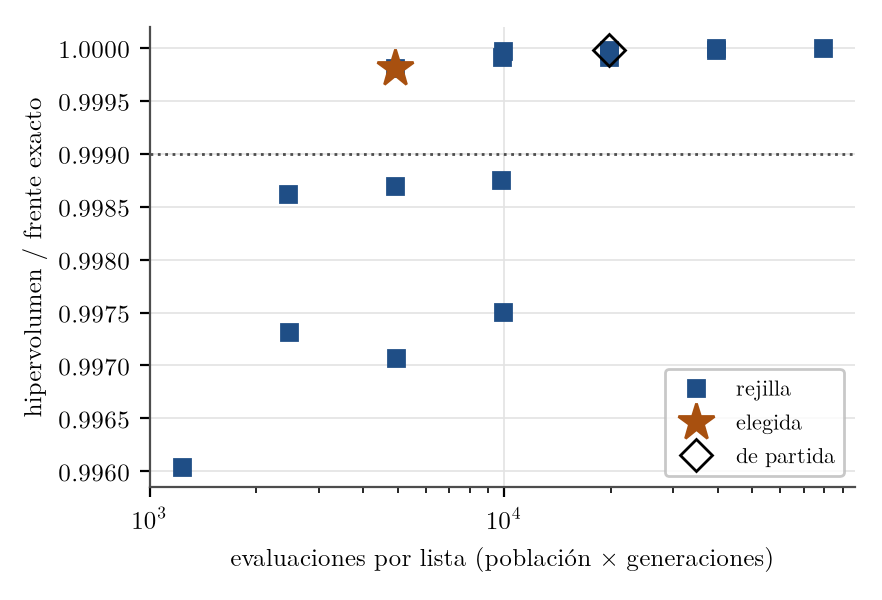
\includegraphics[width=0.7\linewidth]{rejilla.png}
\caption{Hipervolumen relativo contra evaluaciones por lista para cada
configuración de la rejilla; la línea punteada marca el margen de
\calUmbralHV{} bajo el mejor. Fuente: \texttt{calibracion\_nsga.json},
$n=\calCVListas$ listas; los valores están en la \cref{tab:calopt-rejilla}.}
\label{fig:calopt-rejilla}
\end{figure}

El conjunto de prueba se usó una sola vez, con \calSemillasPrueba{} semillas
por lista, para comparar la configuración elegida con la de partida. La
elegida obtuvo un hipervolumen relativo medio de \calPruebaElegidaHV{} (mínimo
por lista \calPruebaElegidaHVMin) contra \calPruebaActualHV{} de la de partida.
La diferencia media es \calDifHV{}, con intervalo bootstrap del 95\,\%
[\calDifHVBajo; \calDifHVAlto] y $p=\calDifHVp$ en la prueba de rangos con
signo de Wilcoxon \cite{wilcoxon_individual_1945}. La pérdida es pequeña pero
real: en prueba la elegida queda algo más lejos del mejor que en la
validación, porque las listas de prueba son algo más grandes (con la configuración de
partida usan \calPruebaActualEvals{} evaluaciones medias, contra
\calEvalsCVPartida{} en la validación) y el margen de \calUmbralHV{} se fijó
sobre otras listas. A cambio, el tiempo medio por
lista bajó de \calPruebaActualT~s a \calPruebaElegidaT~s (diferencia
\calDifT~s, intervalo [\calDifTBajo; \calDifTAlto], $p=\calDifTp$), porque las
evaluaciones medias pasaron de \calPruebaActualEvals{} a
\calPruebaElegidaEvals. El \calFraccionHV{} de las corridas de la elegida
alcanzó al menos 0,999 del hipervolumen exacto, y la peor corrida llegó a
\calRazonMinPrueba.

\paragraph{Umbral de similitud $\tau$.} La resolución acepta sin revisión un
emparejamiento cuyo parecido supera $\tau=0{,}75$. Calibrarlo exige decisiones
humanas, y la base no las tiene: la tabla de transiciones registra
\calTauTransiciones{} resoluciones, todas automáticas y todas con parecido 1.
La única fuente humana es la curaduría de 4 anotadores con una pauta común, que se une con
\calTauPares{} renglones de \calTauListas{} listas de \calTauColegios{}
colegios, y uno solo de ellos aporta \calTauColegioMayor{} renglones. El
parecido solo toma \calTauValores{} valores distintos. Con esos datos, en
$\tau=0{,}75$ se acepta el \calTauAceptada{} de los renglones con una precisión
del \calTauPrecision, y la validación cruzada agrupada elige valores entre
\calTauCVMin{} y \calTauCVMax{} según el pliegue. Por eso $\tau$ se mantiene en
0,75 y se declara como no calibrado.

\paragraph{Sensibilidad del kit recomendado.} Para medir cuánto depende la
recomendación de los pesos, en las \calSensListas{} listas de prueba con al
menos dos puntos en el frente (mediana de \calSensFrenteMediana{} puntos) se
sortearon \calSensPerturbaciones{} vectores de pesos por lista. Sin sobreprecio la estabilidad es 1 por construcción, porque la cota
$f_1\leq(1+\sigma)\min_{\mathcal{P}}f_1$ con $\sigma=0$ deja admisible solo el
kit más barato; las cifras útiles son las de $\sigma>0$. En el primer esquema
cada peso se sortea uniforme dentro de su intervalo del 95\,\% de la P21 y se
renormaliza. Con $\sigma>0$ el kit recomendado fue el mismo en una fracción
media de al menos \calSensICMin{} de los sorteos, aunque en alguna lista bajó
hasta \calSensICMinLista. En el segundo esquema los pesos siguen una Dirichlet
centrada en los de la P21 con concentración $\kappa$, que permite
perturbaciones más anchas que el intervalo; con la más ancha
($\kappa=\calSensKappaMin$) la fracción media no bajó de
\calSensKappaMinEstable. En consecuencia, dentro de lo que la encuesta no
puede descartar la recomendación casi no cambia, y solo se vuelve sensible
cuando el sobreprecio admitido abre muchos kits y los pesos se alejan de los
medidos. La \cref{tab:calopt-sensibilidad} da todas las celdas
y la \cref{fig:calopt-sensibilidad} las muestra.

\begin{table}[htbp]
\centering
\caption{Fracción de sorteos de pesos en que el kit recomendado por MAUT es el
mismo que con los pesos de la P21. DE: desviación estándar del peso del precio
bajo la perturbación. Fuente: \texttt{sensibilidad.json}; $n=\calSensListas$
listas de prueba, \calSensPerturbaciones{} sorteos por lista y celda.}
\label{tab:calopt-sensibilidad}
\small
\begin{tabular}{rlrrlr}
\toprule
sobreprecio & perturbación & DE & media & IC 95\,\% & mínimo por lista \\
\midrule
0\,\% & IC 95\,\% P21 & --- & 1{,}000 & [1{,}000; 1{,}000] & 1{,}000 \\
5\,\% & IC 95\,\% P21 & --- & 0{,}965 & [0{,}932; 0{,}991] & 0{,}610 \\
10\,\% & IC 95\,\% P21 & --- & 0{,}986 & [0{,}964; 1{,}000] & 0{,}692 \\
20\,\% & IC 95\,\% P21 & --- & 0{,}946 & [0{,}904; 0{,}981] & 0{,}540 \\
0\,\% & Dirichlet $\kappa=20$ & 0{,}099 & 1{,}000 & [1{,}000; 1{,}000] & 1{,}000 \\
5\,\% & Dirichlet $\kappa=20$ & 0{,}099 & 0{,}892 & [0{,}830; 0{,}947] & 0{,}429 \\
10\,\% & Dirichlet $\kappa=20$ & 0{,}099 & 0{,}868 & [0{,}822; 0{,}913] & 0{,}541 \\
20\,\% & Dirichlet $\kappa=20$ & 0{,}099 & 0{,}735 & [0{,}663; 0{,}803] & 0{,}168 \\
0\,\% & Dirichlet $\kappa=50$ & 0{,}063 & 1{,}000 & [1{,}000; 1{,}000] & 1{,}000 \\
5\,\% & Dirichlet $\kappa=50$ & 0{,}063 & 0{,}918 & [0{,}866; 0{,}965] & 0{,}502 \\
10\,\% & Dirichlet $\kappa=50$ & 0{,}063 & 0{,}927 & [0{,}888; 0{,}960] & 0{,}558 \\
20\,\% & Dirichlet $\kappa=50$ & 0{,}063 & 0{,}828 & [0{,}765; 0{,}886] & 0{,}287 \\
0\,\% & Dirichlet $\kappa=100$ & 0{,}045 & 1{,}000 & [1{,}000; 1{,}000] & 1{,}000 \\
5\,\% & Dirichlet $\kappa=100$ & 0{,}045 & 0{,}931 & [0{,}884; 0{,}974] & 0{,}520 \\
10\,\% & Dirichlet $\kappa=100$ & 0{,}045 & 0{,}953 & [0{,}923; 0{,}978] & 0{,}618 \\
20\,\% & Dirichlet $\kappa=100$ & 0{,}045 & 0{,}876 & [0{,}818; 0{,}926] & 0{,}379 \\
0\,\% & Dirichlet $\kappa=200$ & 0{,}032 & 1{,}000 & [1{,}000; 1{,}000] & 1{,}000 \\
5\,\% & Dirichlet $\kappa=200$ & 0{,}032 & 0{,}945 & [0{,}903; 0{,}980] & 0{,}557 \\
10\,\% & Dirichlet $\kappa=200$ & 0{,}032 & 0{,}973 & [0{,}946; 0{,}993] & 0{,}632 \\
20\,\% & Dirichlet $\kappa=200$ & 0{,}032 & 0{,}910 & [0{,}857; 0{,}956] & 0{,}456 \\
\bottomrule

\end{tabular}
\end{table}

\begin{figure}[htbp]
\centering
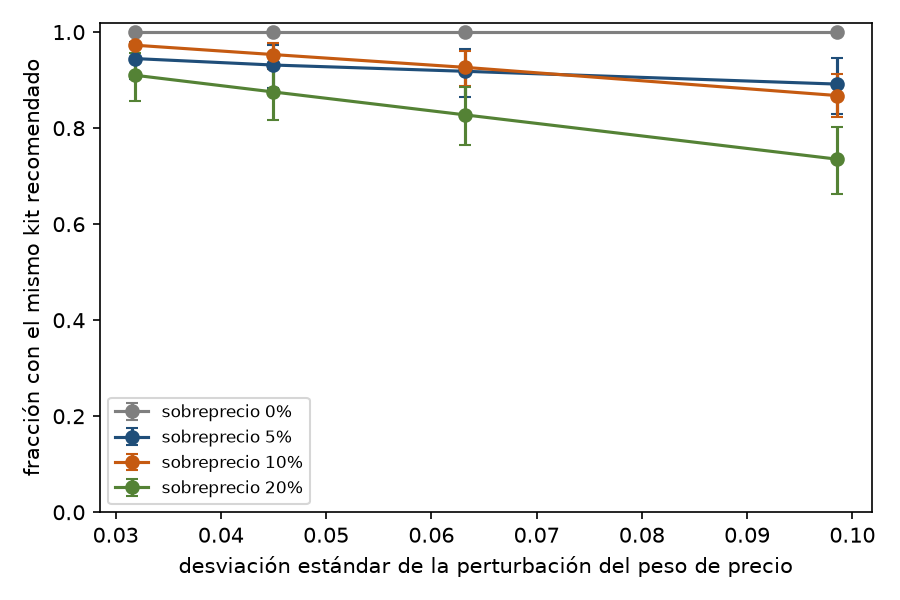
\includegraphics[width=0.7\linewidth]{sensibilidad.png}
\caption{Estabilidad del kit recomendado bajo la perturbación Dirichlet, según
la desviación estándar del peso del precio y el sobreprecio declarado. Fuente:
\texttt{sensibilidad.json}, $n=\calSensListas$ listas; los valores están en la
\cref{tab:calopt-sensibilidad}.}
\label{fig:calopt-sensibilidad}
\end{figure}

\paragraph{Hipervolumen por perfil.} Sobre las \calHVListas{} listas de prueba
(\calHVListasNsga{} de ellas con NSGA-II), el frente de producción alcanzó en
promedio \calHVFrente{} del hipervolumen exacto, con intervalo
[\calHVFrenteBajo; \calHVFrenteAlto] y mínimo \calHVFrenteMin. Cada kit por
separado domina una fracción menor, porque un solo punto no cubre el frente: la
\cref{tab:calopt-hv} da la fracción que domina cada perfil y la
\cref{fig:calopt-hv} la muestra.

\begin{table}[htbp]
\centering
\caption{Hipervolumen relativo al frente exacto en las listas de prueba.
Fuente: \texttt{hipervolumen\_prueba.json}; $n=\calHVListas$ listas.}
\label{tab:calopt-hv}
\small
\begin{tabular}{lrl}
\toprule
conjunto & media & IC 95\,\% \\
\midrule
Frente de producci\'on & 0{,}9969 & [0{,}9951; 0{,}9986] \\
Ahorrador $\cup$ Premium & 0{,}501 & [0{,}474; 0{,}526] \\
Ahorrador & 0{,}362 & [0{,}343; 0{,}382] \\
Premium & 0{,}231 & [0{,}201; 0{,}262] \\
MAUT con pesos P21 & 0{,}517 & [0{,}474; 0{,}558] \\
\bottomrule

\end{tabular}
\end{table}

\begin{figure}[htbp]
\centering
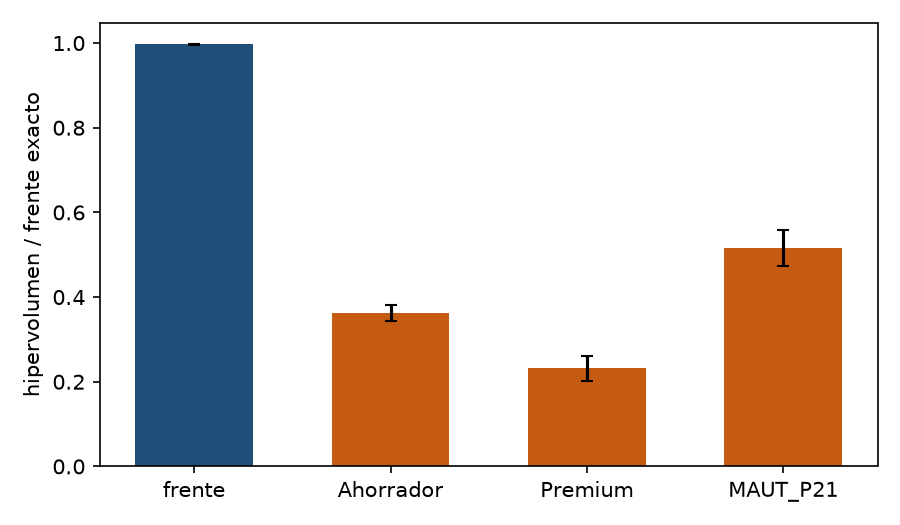
\includegraphics[width=0.6\linewidth]{hipervolumen_prueba.png}
\caption{Hipervolumen relativo del frente de producción y de cada kit. Fuente:
\texttt{hipervolumen\_prueba.json}, $n=\calHVListas$ listas; los valores están
en la \cref{tab:calopt-hv}.}
\label{fig:calopt-hv}
\end{figure}

\paragraph{Constantes.} La \cref{tab:calopt-constantes} reúne el valor de cada
constante, su fuente y la evidencia que la sostiene.

\begin{table}[htbp]
\centering
\caption{Constantes del optimizador, con su fuente y su evidencia.}
\label{tab:calopt-constantes}
\small
\begin{tabular}{p{0.14\linewidth}p{0.33\linewidth}p{0.16\linewidth}p{0.25\linewidth}}
\toprule
constante & valor & fuente & evidencia \\
\midrule
Pesos por omisión & \calWPrecio; \calWMarca; \calWCalidad; \calWPersonaje &
P21, $n=\calEncuestados$ & IC 95\,\% bootstrap en el texto \\
Umbral $\Lambda$ & $\calLimite=2^{\calLimiteLog}$ & \cref{tab:calopt-umbral} &
cruce medido en $2^{\calCruceElegidaLog}$ (mediana) y $2^{\calCruceElegidaPLog}$ (percentil 95) \\
Población $N$ & $\mathrm{par}(\min(\calPobProdMax,\max(\calPobProdMin,\calPobProdLinea\,n)))$, $a=\calA$ &
\cref{tab:calopt-rejilla} & validación agrupada, \calPlieguesIguales{} pliegues coinciden \\
Generaciones $G$ & $\min(\calGenProdMax,\max(\calGenProdMin,\calGenProdDecada\log_{10}S))$, $b=\calB$ &
\cref{tab:calopt-rejilla} & prueba: HV \calPruebaElegidaHV{}, diferencia \calDifHV \\
$\tau$ & 0,75 (sin calibrar) & curaduría de 4 anotadores & $n=\calTauPares$ renglones, \calTauColegios{} colegios \\
\bottomrule
\end{tabular}
\end{table}

\paragraph{Amenazas a la validez.} Los resultados anteriores tienen seis
limitaciones, que se declaran para que se lean con su alcance.

\begin{enumerate}[label=\textbf{A\arabic*.}]
  \item \emph{Preferencias declaradas.} Los pesos salen de lo que
  \calEncuestados{} acudientes dicen, no de lo que compran, y la muestra es
  sobre todo de estrato 4. Los intervalos de la P21 son anchos para su tamaño
  y no permiten ordenar los tres primeros criterios entre sí.
  \item \emph{Corpus pequeño y agrupado.} Hay \calListas{} listas de
  \calColegios{} colegios. Por eso la partición se hizo por colegio, y el
  conjunto de prueba tiene solo \calColegiosPrueba{} colegios.
  \item \emph{$\tau$ sin calibrar.} No hay decisiones humanas registradas en la
  base: las \calTauTransiciones{} resoluciones son automáticas y todas tienen
  parecido 1. La única fuente es la curaduría de 4 anotadores, concentrada en un
  colegio. $\tau$ se deja en su valor por omisión.
  \item \emph{No existe un kit óptimo de referencia.} El hipervolumen mide qué
  tan bien se resuelve el problema de optimización, no si el kit le sirve al
  acudiente. Esa pregunta la responde la validación con usuarios (OE5).
  \item \emph{Calibración retrospectiva.} La calibración usó listas ya
  recolectadas. El conjunto de prueba se apartó antes y se usó una sola vez,
  pero no reemplaza una evaluación con listas nuevas.
  \item \emph{Una sola máquina.} Los tiempos se midieron en un \calCPU{} con
  \calRAM~GiB. En otra máquina cambian las constantes del ajuste y con ellas el
  cruce, aunque no el exponente ni el orden de las curvas.
\end{enumerate}
